\documentclass[10pt,letterpaper,oneside]{article}
\usepackage[T1]{fontenc}
\usepackage[utf8]{inputenc}
\usepackage{lmodern}
\usepackage{geometry}
\geometry{margin=0.84in,headheight=21pt,footskip=28pt}
\usepackage{microtype}
\usepackage{xcolor}
\definecolor{ink}{HTML}{15253D}
\definecolor{accent}{HTML}{086A84}
\definecolor{pale}{HTML}{EEF5F8}
\definecolor{muted}{HTML}{4E6474}
\definecolor{grayline}{HTML}{D7E2E8}
\usepackage{graphicx}
\usepackage{fancyhdr}
\usepackage{titlesec}
\usepackage{enumitem}
\usepackage{array,tabularx,longtable,booktabs}
\usepackage[most]{tcolorbox}
\usepackage{xurl}
\usepackage{hyperref}
\usepackage{listings}
\usepackage{amsmath,amssymb}
\usepackage{tikz}
\usetikzlibrary{arrows.meta,positioning,shapes.geometric,calc}
\hypersetup{colorlinks=true,linkcolor=accent,urlcolor=accent,pdftitle={Competency Curriculum and Complete Handbook Reference Index},pdfauthor={Independent technical engineering study companion}}
\renewcommand{\familydefault}{\sfdefault}
\linespread{1.07}
\setlength{\parindent}{0pt}
\setlength{\parskip}{5.5pt}
\emergencystretch=2em
\setlist[itemize]{leftmargin=1.5em,itemsep=2.5pt,topsep=3pt}
\setlist[enumerate]{leftmargin=1.7em,itemsep=3pt,topsep=3pt}
\titleformat{\section}{\Large\bfseries\color{ink}}{\thesection}{0.65em}{}[\vspace{-2pt}{\color{accent}\titlerule}]
\titleformat{\subsection}{\large\bfseries\color{accent}}{\thesubsection}{0.6em}{}
\titleformat{\subsubsection}{\bfseries\color{ink}}{\thesubsubsection}{0.6em}{}
\titlespacing*{\section}{0pt}{16pt}{9pt}
\titlespacing*{\subsection}{0pt}{11pt}{6pt}
\pagestyle{fancy}\fancyhf{}\fancyhead[L]{\footnotesize\color{muted} COMPUTER \& INFORMATION SECURITY ENGINEERING}\fancyhead[R]{\footnotesize\color{accent} SUITE / 8}\fancyfoot[L]{\footnotesize\color{muted} Independent study companion \quad|\quad 2026}\fancyfoot[R]{\footnotesize\color{muted}\thepage}\renewcommand{\headrulewidth}{0.4pt}\renewcommand{\headrule}{\hbox to\headwidth{\color{grayline}\leaders\hrule height \headrulewidth\hfill}}
\newtcolorbox{sourcebox}{enhanced,breakable,boxrule=0pt,leftrule=3pt,colframe=accent,colback=pale,arc=0pt,left=9pt,right=7pt,top=7pt,bottom=7pt}
\newtcolorbox{warningbox}{enhanced,breakable,boxrule=0.5pt,colframe=grayline,colback=white,arc=1pt,left=9pt,right=9pt,top=7pt,bottom=7pt}
\newcommand{\handbookref}[1]{\textsf{\color{accent}\textbf{[H:#1]}}}
\newcommand{\modernext}{\textsf{\color{muted}\textbf{[E]}}}
\newcommand{\designed}{\textsf{\color{accent}\textbf{[D]}}}
\newcommand{\deliverable}[1]{\textbf{Deliverable:} #1}
\lstdefinestyle{lab}{basicstyle=\ttfamily\scriptsize,keywordstyle=\color{accent}\bfseries,commentstyle=\color{muted},numbers=left,numberstyle=\tiny\color{muted},numbersep=7pt,breaklines=true,showstringspaces=false,frame=single,rulecolor=\color{grayline},backgroundcolor=\color{pale},xleftmargin=1em,framexleftmargin=0.6em,tabsize=2,columns=fullflexible}
\lstset{style=lab}
\renewcommand{\arraystretch}{1.21}
\newcommand{\makereportcover}[4]{%
\thispagestyle{empty}\vspace*{1.15in}
{\small\bfseries\color{accent} COMPUTER AND INFORMATION SECURITY ENGINEERING}\par\vspace{13pt}
{\Huge\bfseries\color{ink} #1\par}\vspace{15pt}
{\Large\color{muted} #2\par}\vspace{18pt}
\color{accent}\rule{0.94\textwidth}{2.1pt}\par\vspace{20pt}
{\normalsize\bfseries Document #3 of 8 \quad\textbullet\quad 16 October 2026\par}
\vspace{0.35in}
\begin{sourcebox}\textbf{Orientation.} #4\end{sourcebox}
\vfill
{\small\color{muted} Independent, original engineering study and practice materials grounded in\par
\emph{Computer and Information Security Handbook}, 4th ed., edited by John R. Vacca,\par
Elsevier/Morgan Kaufmann, 2025, Volumes I--II. Not a reproduction or official standard.}
\newpage\setcounter{page}{1}\tableofcontents\newpage
}
\begin{document}
\makereportcover{Competency Curriculum and Complete Handbook Reference Index}{Prerequisite learning graph, 16-week plan, role tracks, capstone and 104-chapter coverage}{8}{A complete learning program with chapter-to-document coverage across both handbook volumes, staged practice, assessment rubrics, and role-specific progression.}

\section{Use of this curriculum}
This curriculum reorganizes the handbook's 104 chapters for cumulative technical competence while preserving their original chapter identities. It is an independent instructional design, not the publisher's official course or a replacement for the full text. Each stage names reading anchors, original deliverables and observable assessment.

\section{Competency graph: learn dependencies before tools}
\begin{center}
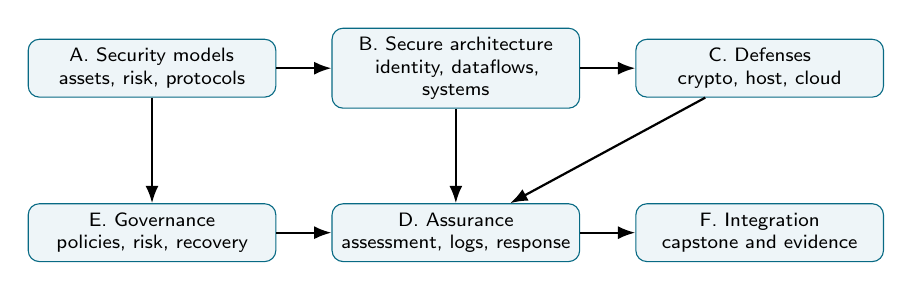
\begin{tikzpicture}[node distance=4mm and 7mm,every node/.style={font=\scriptsize}, task/.style={draw=accent,rounded corners,fill=pale,text width=0.24\textwidth,minimum height=0.68cm,align=center}]
\node[task] (a) {A. Security models\\assets, risk, protocols};
\node[task,right=of a] (b) {B. Secure architecture\\identity, dataflows, systems};
\node[task,right=of b] (c) {C. Defenses\\crypto, host, cloud};
\node[task,below=12mm of b] (d) {D. Assurance\\assessment, logs, response};
\node[task,left=of d] (e) {E. Governance\\policies, risk, recovery};
\node[task,right=of d] (f) {F. Integration\\capstone and evidence};
\draw[-{Latex[length=2.2mm]},thick] (a)--(b);
\draw[-{Latex[length=2.2mm]},thick] (b)--(c);
\draw[-{Latex[length=2.2mm]},thick] (a)--(e);
\draw[-{Latex[length=2.2mm]},thick] (b)--(d);
\draw[-{Latex[length=2.2mm]},thick] (c)--(d);
\draw[-{Latex[length=2.2mm]},thick] (e)--(d);
\draw[-{Latex[length=2.2mm]},thick] (d)--(f);
\end{tikzpicture}
\end{center}
\handbookref{1--104} \designed{} Suggested preparation: basic TCP/IP; Linux shell; application development; IAM concepts; mathematical functions/keys; standard source control. Students who lack a prerequisite complete remediation work before advancing.

\section{Sixteen-week instructional plan}
\par\medskip\noindent\begin{longtable}{@{}p{0.11\textwidth}p{0.27\textwidth}p{0.26\textwidth}p{0.26\textwidth}@{}}\toprule
Weeks & Domain / chapters & Practice artifact & Gate \\ \midrule\endhead
1--2 & Fundamentals, assets, threats; Chs.~1--8, 24, 28--29, 35 & Asset inventory, dataflow, risk scenarios & Explain threat/control/evidence distinctions\\
3--4 & Networks, Linux, web; Chs.~10--18, 75--80 & Segmentation and host hardening review & Negative access test and traffic analysis\\
5--6 & Cryptography, PKI, IAM; Chs.~3--4, 47--61, 72--73, 82 & Key inventory and identity flow & Explain chain validation and authZ gaps\\
7--8 & Secure/cloud architecture; Chs.~9, 19--23, 62--70, 83, 89--93 & Architecture views, ADR and fault model & Traceable controls and recovery assumptions\\
9--10 & Governance, metrics, recovery; Chs.~25--27, 33--40, 81 & Risk register, policy and BIA & Approved owners, evidence and test plan\\
11--12 & Assessment, defense and DFIR; Chs.~5--8, 31--32, 41--46, 74--77 & Triage dossier, incident timeline & Evidence preservation and fixed issue retested\\
13--14 & Specialized domains and AI; Chs.~83--104 & Sector-specific control delta and AI misuse review & Safety/privacy and novel-risk reasoning\\
15 & Integration & Capstone design and implementation & Peer review and controlled security test\\
16 & Validation and communication & Capstone evidence dossier and defense & Final rubric and oral review\\
\bottomrule\end{longtable}\par\medskip
Timing assumes 6--10 hours weekly and instructor feedback; adjust for prerequisites and operational access. \designed{}

\section{Mastery outcomes by engineering role}
\par\medskip\noindent\begin{tabularx}{\textwidth}{@{}p{0.20\textwidth}X X@{}}\toprule
Role track & Depth emphasis & Measured evidence \\ \midrule
Security architect & Trust boundaries, systemic risk, cloud/OT patterns & Four architecture views and signed ADRs\\
Application security engineer & API auth, taint, SAST, SCA, triage & Mapped CWE paths, tests and closure package\\
Detection/SOC engineer & NSM, log pipelines, incidents, coverage & Validated detection and response runbook\\
Governance/risk lead & Risk owners, controls, metrics, BIA & Decision-ready risk dashboard and test packet\\
Cloud/platform engineer & IAM, infrastructure config, secret and key lifecycle & Repeatable baseline and rollback proof\\
Forensic investigator & Acquisition, integrity, provenance & Defensible chronology and custody records\\
\bottomrule\end{tabularx}\par\medskip
\designed{} Common foundations are mandatory; role tracks change depth, not authorization requirements.

\section{Assessment design and learning evidence}
\subsection{Three assessment formats}\designed{}
\begin{enumerate}
\item \textbf{Knowledge check (20\%):} scenario-based written questions, not trivia about tool syntax.
\item \textbf{Practical lab (40\%):} repeatable tests, controlled environment, failure evidence and rollback.
\item \textbf{Architecture/incident defense (40\%):} traceable decisions, tradeoffs and peer challenge.
\end{enumerate}
Minimum overall score is 80\%. Independently require pass on scope/authorization, critical authorization invariants and evidence integrity; strong averages do not compensate for unsafe conduct. Students who fail one gate complete corrective work and a new verification trial.
\subsection{Bloom-style progression}\designed{}
\textbf{Explain}: distinguish risk, vulnerability and impact. \textbf{Apply}: write an authorization test. \textbf{Analyze}: compare logs against a threat hypothesis. \textbf{Evaluate}: justify risk acceptance under uncertainty. \textbf{Create}: produce a reviewable architecture, evidence package and migration plan.

\section{Integrated capstone: connected-service platform}
Design a multi-tenant web service that reads IoT sensor measurements, exposes user dashboards, stores events in a cloud database, and provides limited remote device management. Threats include credential theft, cross-tenant disclosure, unsafe device instructions, supply-chain defects, cloud storage errors and loss of telemetry.
\subsection{Required deliverables}\designed{}
\begin{enumerate}
\item System-context, trust-boundary, deployment and recovery views.
\item Asset register and at least 12 scenario-based threat statements.
\item Fifteen numbered security requirements with testable acceptance criteria.
\item Identity and authorization contract, key inventory and privacy processing inventory.
\item Risk register with treatment owners and at least four residual-risk decisions.
\item Controlled negative tests for tenancy, device authorization, data validation and recovery.
\item One detection with normal/abnormal cases and a sample triage runbook.
\item A vulnerability finding, fix, verification record and evidence manifest.
\item An incident tabletop and custody-safe timeline.
\item An executive summary containing scope, major residual risks, decisions and next actions.
\end{enumerate}
\subsection{Scoring}
\par\medskip\noindent\begin{tabularx}{\textwidth}{@{}p{0.38\textwidth}X@{}}\toprule
Dimension & Weight and required proof \\ \midrule
Requirements and architecture traceability & 20: every critical requirement has a control and test\\
Security properties and tenant isolation & 20: negative tests demonstrate object-level enforcement\\
Operational resilience and observability & 15: recovery and detection exercises with metrics\\
Risk and governance quality & 15: explicit risk owners and defensible exceptions\\
Evidence, reproducibility and safe scope & 20: versioned artifact set and chain of custody\\
Communication & 10: concise technical and management reporting\\
\bottomrule\end{tabularx}\par\medskip

\section{Handbook-to-suite coverage protocol}
The following register provides an original, \emph{one-primary-document} assignment for each of the 104 handbook chapters. It does not imply that a chapter is exhaustively reproduced in the listed document: the original handbook contains much deeper treatment. Primary document is where a learner first applies the chapter's subject; cross-cutting topics appear in several volumes. Chapter PDF-page references correspond to the supplied combined PDF, not publisher-printed page numbers.
\begin{sourcebox}\textbf{Reading protocol:} locate the chapter using the identifier and combined-PDF start page; read its definitions and worked examples; note edition-specific/legacy technologies; compare to the suite's labeled contemporary extensions; complete the applicable evidence task. \designed{}\end{sourcebox}
\small\par\medskip\noindent\begin{longtable}{@{}p{0.065\textwidth}p{0.61\textwidth}p{0.095\textwidth}p{0.12\textwidth}@{}}\toprule Ch. & Source chapter (both volumes) & PDF page & Primary doc. \\ \midrule\endhead\bottomrule\endfoot
1 & Information Security in the Modern Enterprise & 39 & 1 \\
2 & Building a Secure Organization & 49 & 1 \\
3 & A Cryptography Primer & 59 & 5 \\
4 & Verifying User and Host Identity & 83 & 1 \\
5 & Detecting System Intrusions & 91 & 4 \\
6 & Intrusion Detection in Contemporary Environments & 135 & 4 \\
7 & Preventing System Intrusions & 157 & 1 \\
8 & Guarding Against Network Intrusions & 175 & 4 \\
9 & Fault Tolerance and Resilience in Cloud Computing Environments & 191 & 2 \\
10 & Securing Web Applications, Services, and Servers & 211 & 2 \\
11 & UNIX and Linux Security & 233 & 2 \\
12 & Eliminating the Security Weakness of Linux and UNIX Operating Systems & 253 & 2 \\
13 & Internet Security & 271 & 4 \\
14 & The Botnet Problem & 297 & 1 \\
15 & Intranet Security & 309 & 4 \\
16 & Local Area Network Security & 331 & 4 \\
17 & Wireless Network Security & 351 & 2 \\
18 & Wireless Sensor Network Security: The Internet of Things & 367 & 2 \\
19 & Security for the Internet of Things & 389 & 2 \\
20 & Cellular Network Security & 405 & 2 \\
21 & Radio Frequency Identification Security & 425 & 2 \\
22 & Optical Network Security & 443 & 2 \\
23 & Optical Wireless Security & 451 & 2 \\
24 & Information Security Essentials for IT Managers: Protecting Mission-Critical Systems & 459 & 3 \\
25 & Security Management Systems & 469 & 3 \\
26 & Policy-Driven System Management & 477 & 3 \\
27 & Information Technology Security Management & 511 & 3 \\
28 & The Enemy (The Intruder's Genesis) & 545 & 1 \\
29 & Social Engineering Deceptions and Defenses & 557 & 1 \\
30 & Hacking in an Ethical Way & 567 & 6 \\
31 & What Is Vulnerability Assessment? & 573 & 6 \\
32 & Introduction to Vulnerabilities Below the Operating System & 585 & 6 \\
33 & Security Metrics: An Introduction and Literature Review & 595 & 3 \\
34 & Security Education, Training, and Awareness & 609 & 3 \\
35 & Risk Management & 619 & 3 \\
36 & Insider Threats & 637 & 1 \\
37 & Disaster Recovery & 651 & 3 \\
38 & Disaster Recovery Plans for Small and Medium Business (SMB) & 661 & 3 \\
39 & Security Certification and Standards Implementation & 671 & 3 \\
40 & Security Policies and Plans Development & 679 & 3 \\
41 & Cyber Forensics & 687 & 6 \\
42 & Cyber Forensics and Incidence Response & 717 & 6 \\
43 & Securing e-Discovery & 743 & 6 \\
44 & Network Forensics & 769 & 6 \\
45 & Microsoft Office and Metadata Forensics: A Deeper Dive & 785 & 6 \\
46 & Hard Drive Imaging & 795 & 6 \\
47 & Data Encryption & 801 & 5 \\
48 & Satellite Encryption & 827 & 5 \\
49 & Public Key Infrastructure & 841 & 5 \\
50 & Password-Based Authenticated Key Establishment Protocols & 863 & 5 \\
51 & Context-Aware Multifactor Authentication Survey & 879 & 5 \\
52 & Instant-Messaging Security & 891 & 5 \\
53 & Online Privacy & 957 & 5 \\
54 & Privacy-Enhancing Technologies & 977 & 5 \\
55 & Personal Privacy Policies & 993 & 5 \\
56 & Detection of Conflicts in Security Policies & 1003 & 5 \\
57 & Supporting User Privacy Preferences in Digital Interactions & 1023 & 5 \\
58 & Privacy and Security in Environmental Monitoring Systems: Issues and Solutions & 1045 & 5 \\
59 & Virtual Private Networks & 1065 & 5 \\
60 & Identity Theft & 1079 & 5 \\
61 & VoIP Security & 1093 & 5 \\
62 & SAN Security & 1111 & 2 \\
63 & Storage Area Networking Security Devices & 1135 & 2 \\
64 & Securing Cloud Computing Systems & 1151 & 4 \\
65 & Cloud Security & 1167 & 4 \\
66 & Cloud Security Trends & 1179 & 4 \\
67 & Private Cloud Security & 1195 & 4 \\
68 & Virtual Private Cloud Security & 1203 & 4 \\
69 & Protecting Virtual Infrastructure & 1211 & 2 \\
70 & Software-Defined Networking and Network Function Virtualization Security & 1219 & 2 \\
71 & Physical Security & 1231 & 1 \\
72 & Biometrics & 1247 & 5 \\
73 & Online Identity and User Management Services & 1265 & 5 \\
74 & Intrusion Prevention and Detection Systems & 1289 & 4 \\
75 & Transmission Control Protocol/Internet Protocol Packet Analysis & 1303 & 4 \\
76 & Firewalls & 1317 & 4 \\
77 & Penetration Testing & 1337 & 6 \\
78 & System Security & 1345 & 4 \\
79 & Access Controls & 1353 & 5 \\
80 & Endpoint Security & 1361 & 4 \\
81 & Assessments and Audits & 1369 & 3 \\
82 & Fundamentals of Cryptography & 1377 & 5 \\
83 & Securing the Infrastructure & 1387 & 2 \\
84 & Cyberattacks Against the Grid Infrastructure & 1401 & 4 \\
85 & Energy Infrastructure Cyber Security & 1409 & 4 \\
86 & Homeland Security and Cybersecurity & 1417 & 4 \\
87 & Cyber Warfare & 1431 & 4 \\
88 & Cyber Attack Process & 1467 & 1 \\
89 & Smart Cities: Cybersecurity Concerns & 1483 & 2 \\
90 & Disaster Management Cycle, Smart Technologies, Urban Form, Traditional Developments, and Sprawl & 1499 & 2 \\
91 & Cyber Security in Smart Homes & 1523 & 2 \\
92 & Future Trends for Cyber Security for Smart Cities and Homes & 1543 & 2 \\
93 & An Overview of Cyber Attacks and Defenses on Intelligent Connected Vehicles & 1567 & 2 \\
94 & Security Through Diversity & 1583 & 7 \\
95 & Online e-Reputation Management Services & 1595 & 3 \\
96 & Content Filtering & 1607 & 7 \\
97 & Data Loss Protection & 1629 & 6 \\
98 & Satellite Cyber Attack Search and Destroy & 1647 & 4 \\
99 & Verifiable Voting Systems & 1667 & 7 \\
100 & Advanced Data Encryption & 1691 & 5 \\
101 & Use of Artificial Intelligence (AI) in Cybersecurity & 1703 & 6 \\
102 & AI Abuse: Investigating the Threat Landscape & 1711 & 1 \\
103 & Future Trends for Cyber Attacks in the Healthcare Industry & 1737 & 2 \\
104 & Future Trends in Maritime Cybersecurity & 1749 & 2 \\
\end{longtable}\par\medskip\normalsize

\section{Qualification review and maintenance}
Every quarter, instructors should review standards and tool versions, verify lab commands on the supported platform and document substantive changes. Reevaluate AI, cloud, cryptographic and critical-infrastructure assumptions when safety, law, dependency versions or deployment patterns change. \handbookref{92,101--104} \modernext{}
\begin{warningbox}\textbf{Graduation packet:} assessment scores; authorized scope statements; eight laboratory evidence manifests; capstone architecture and risk register; verified findings and fixes; recovery test; incident timeline; instructor feedback and improvement backlog. \designed{}\end{warningbox}


\section*{Source and reference register}
\addcontentsline{toc}{section}{Source and reference register}
\begin{description}[leftmargin=1.6em,style=nextline]
\item[H] John R. Vacca (ed.), \emph{Computer and Information Security Handbook}, 4th ed., Volumes I--II, Elsevier/Morgan Kaufmann, 2025. Chapter identifiers in this document point to this book.
\item[N1] NIST, \emph{Cybersecurity Framework 2.0} (2024), \url{https://www.nist.gov/cyberframework}.
\item[N2] NIST SP 800-218, \emph{Secure Software Development Framework v1.1} (2022), \url{https://csrc.nist.gov/pubs/sp/800/218/final}. Later drafts are not treated as final requirements.
\item[N3] NIST SP 800-61 Rev. 3, \emph{Incident Response Recommendations and Considerations for Cybersecurity Risk Management} (2025), \url{https://csrc.nist.gov/pubs/sp/800/61/r3/final}.
\item[N4] NIST SP 800-63-4, \emph{Digital Identity Guidelines} (2025), \url{https://csrc.nist.gov/pubs/sp/800/63/4/final}.
\item[N5] NIST, FIPS 203/204/205 (2024), \url{https://csrc.nist.gov/Projects/Post-Quantum-Cryptography/publications}.
\item[O1] OWASP, \emph{API Security Top 10} (2023), \url{https://api-security.owasp.org/editions/2023/en/0x11-t10/}.
\item[C1] CISA, \emph{Known Exploited Vulnerabilities Catalog}, \url{https://www.cisa.gov/known-exploited-vulnerabilities-catalog}.
\item[M1] MITRE ATT\&CK Enterprise, \url{https://attack.mitre.org/matrices/enterprise/}.
\item[G1] GitHub, \emph{REST API endpoints for code scanning}, \url{https://docs.github.com/en/rest/code-scanning}.
\end{description}
\begin{warningbox}\textbf{Interpretation rule.} \handbookref{number} identifies a conceptual anchor in the supplied handbook, not a verbatim quotation or an official requirement. \modernext{} identifies a contemporary extension informed by external references or current engineering practice. \designed{} identifies an independently developed example, template, exercise, metric, or operational procedure. Requirements are binding only if separately adopted through applicable law, contract, policy, or the cited standards; this suite does not assert otherwise.\end{warningbox}

\end{document}
